% !TEX root =  centrtutorial.tex

\begin{frame}
  \frametitle{Part 4}
  \centering
  \Huge Scalable Algorithms
\end{frame}


\begin{frame}
  \frametitle{Parallelism}

  \begin{itemize}
    \item Fine grained: single concurrent BFS
    \item Only one copy of auxiliary data structires
    \item Synchronization needed
    \item Better for GPUs, which have small memory
  \end{itemize}
  \begin{itemize}
    \item Coarse grained: many independent BFSs
    \item Sources are independent, embarrassingly parallel
    \item More memory needed
    \item Better for CPUs, which have large memory
  \end{itemize}
\end{frame}
 
 
%% Sariy�ce et al.
\begin{frame}
  \frametitle{Betweenness Centrality on GPUs and Heterogeneous Architectures}
  \centering
  \vfill
  {\huge A. E. Sariy�ce, K. Kaya, E. Saule, �.~V.~�ataly�rek}
  \vfill
  {\large GPGPU '13: Workshop on General Purpose Processing Using GPUs}
\end{frame}


\begin{frame}
  \frametitle{GPU}

  \begin{quote}
    A GPU is especially well-suited to address problems that can be expressed as \textbf{data-parallel computations} - the same program is executed on many data elements in parallel - with \textbf{high arithmetic intensity} - the ratio of arithmetic operations to memory operations.
    
    Because the same program is executed for each data element, there is a lower requirement for sophisticated flow control, and because it is executed on many data elements and has high arithmetic intensity, the memory access latency can be hidden with calculations instead of big data caches.\footnote{\url{http://docs.nvidia.com/cuda/cuda-c-programming-guide/index.html}}
  \end{quote}
\end{frame}


\begin{frame}
  \frametitle{Execution model}
  \begin{columns}[onlytextwidth]

    \begin{column}{0.5\textwidth}
      \begin{itemize}
        \item One thread per data element
        \item Thread scheduled in blocks with barriers (wait for others at the end)
        \item Program runs on the whole data (kernel)
      \end{itemize}
      \begin{itemize}
        \item Minimize synchronization
        \item Balance load
        \item Coalesce memory access
      \end{itemize}
    \end{column}

    \begin{column}{0.5\textwidth}
      \begin{figure}[t]
        \centering
        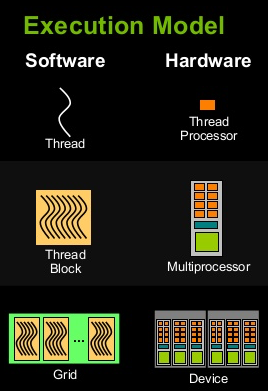
\includegraphics[width=\textwidth, height=0.8\textheight, keepaspectratio]{imgs/cuda}
      \end{figure}
    \end{column}
  \end{columns}
  
\end{frame}


\begin{frame}
  \frametitle{Intuition}

  \begin{itemize}
    \item GPUs have huge number of cores
    \item Use them to parallelize BFS
    \item One core per vertex, or one core per edge
    \item Vertex-based parallelism creates load imbalance for graphs with skewed degree distribution
    \item Edge-based parallelism requires high memory usage
  \end{itemize}
  \begin{itemize}
    \item Use vertex-based parallelism
    \item Virtualize high-degree nodes to address load imbalance
    \item Reduce memory usage by removing predecessors lists
  \end{itemize}
  
\end{frame}


\begin{frame}
  \frametitle{Difference}
  
  \begin{columns}[onlytextwidth]
    \begin{column}{0.5\textwidth}
      \begin{figure}[t]
        \centering
        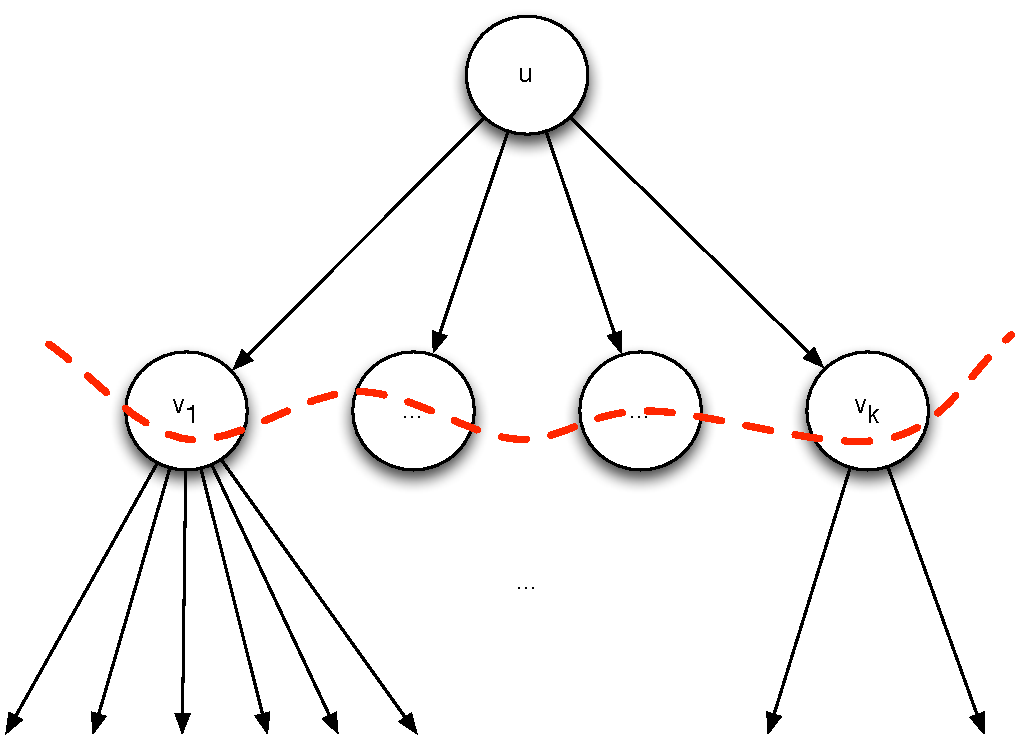
\includegraphics[width=\textwidth, height=0.6\textheight, keepaspectratio]{imgs/gpu-vertex-bfs}
        \caption{Vertex-based BFS}
      \end{figure}
    \end{column}
    
    \begin{column}{0.5\textwidth}
      \begin{figure}[t]
        \centering
        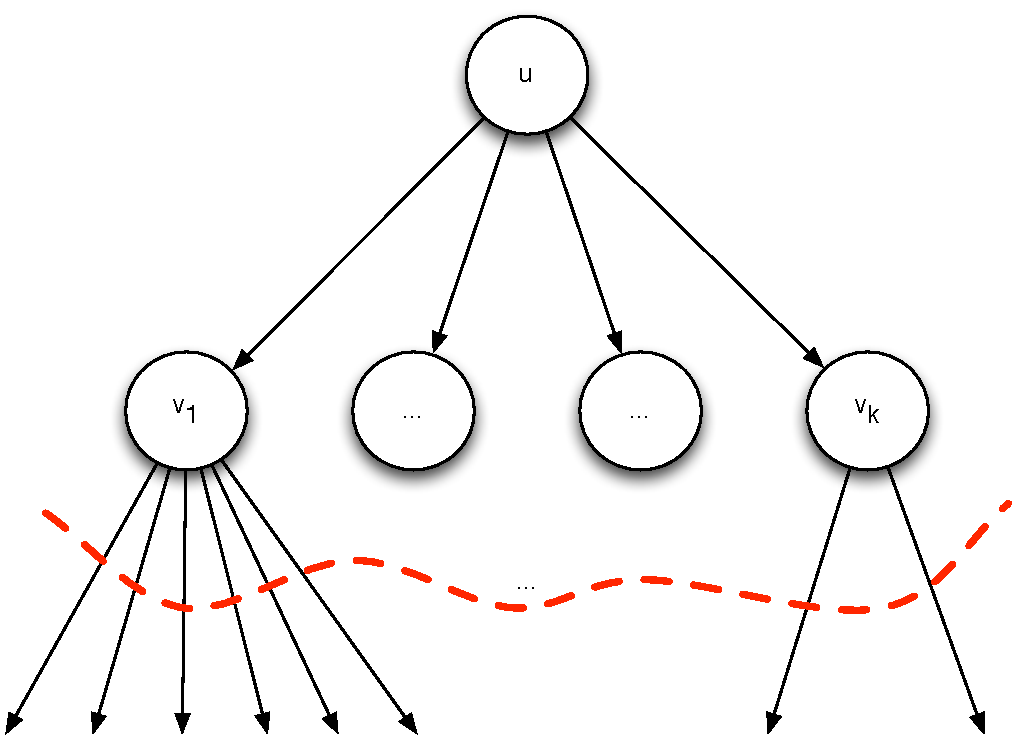
\includegraphics[width=\textwidth, height=0.6\textheight, keepaspectratio]{imgs/gpu-edge-bfs}
        \caption{Edge-based BFS}
      \end{figure}
    \end{column}
  \end{columns}

\end{frame}


\begin{frame}
  \frametitle{Vertex-based}
  
  \begin{columns}[onlytextwidth]
    \begin{column}{0.5\textwidth}
      \begin{itemize}
        \item For each level, for each vertex in parallel
        \item If vertex is on level
        \item For each neighbor, adjust \pred and \paths
        \item Atomic update on \paths needed (multiple paths can be discovered concurrently)
        \item While backtracking, if $u \in \pred(v)$ accumulate $\dep(u) = \dep(u) + \dep(v)$
        \item Possible load imbalance if degree skewed
      \end{itemize}
    \end{column}

    \begin{column}{0.5\textwidth}
      \begin{figure}[t]
        \centering
        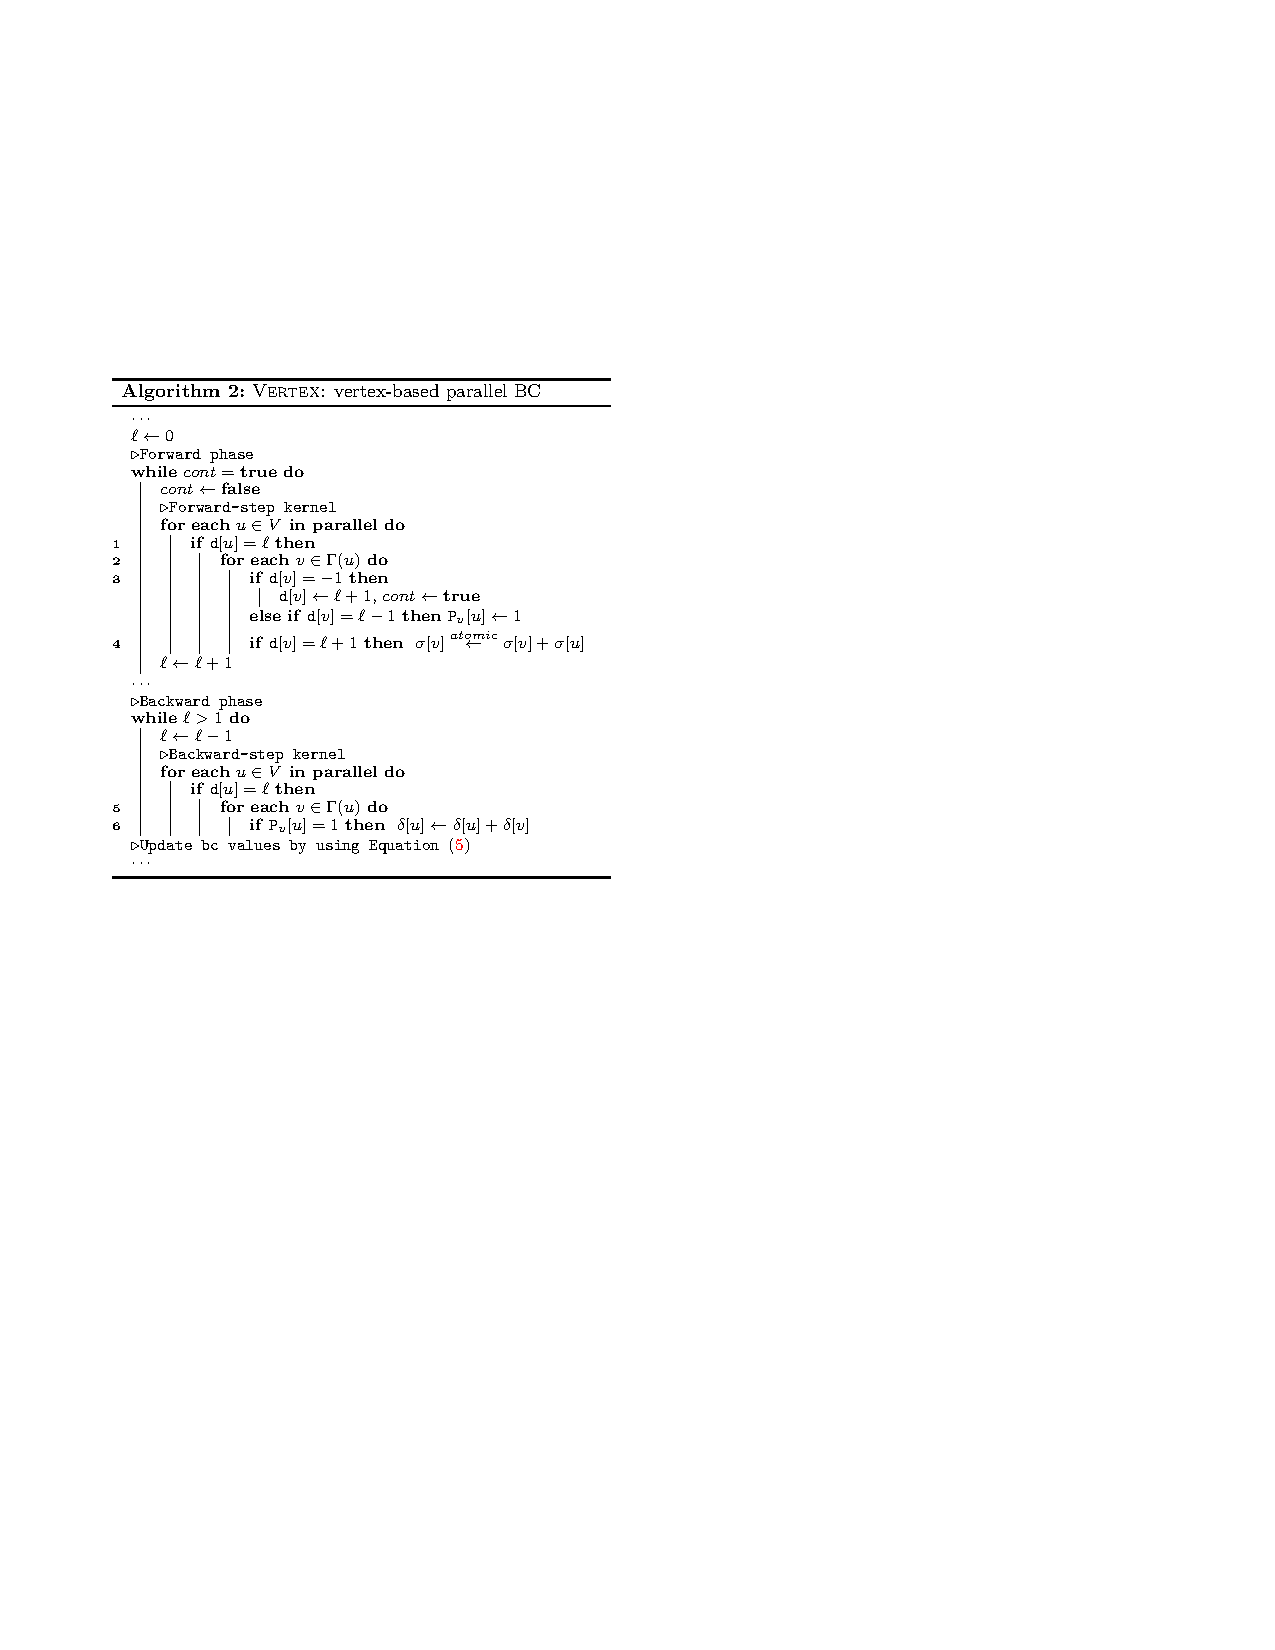
\includegraphics[width=\textwidth, height=0.8\textheight, keepaspectratio]{imgs/gpu-algo-vertex}
      \end{figure}
    \end{column}
  \end{columns}
  
\end{frame}


\begin{frame}
  \frametitle{Edge-based}
  
  \begin{columns}[onlytextwidth]
    \begin{column}{0.5\textwidth}
      \begin{itemize}
        \item For each level, for each edge in parallel
        \item If edge endpoint is on level
        \item Same as above...
        \item While backtracking, if $u \in \pred(v)$ accumulate $\dep(u) = \dep(u) + \dep(v)$ \emph{atomically}
        \item Multiple edges can try to update \dep concurrently
        \item More memory (edge-based layout) \\ and more atomic operations
      \end{itemize}
    \end{column}

    \begin{column}{0.5\textwidth}
      \begin{figure}[t]
        \centering
        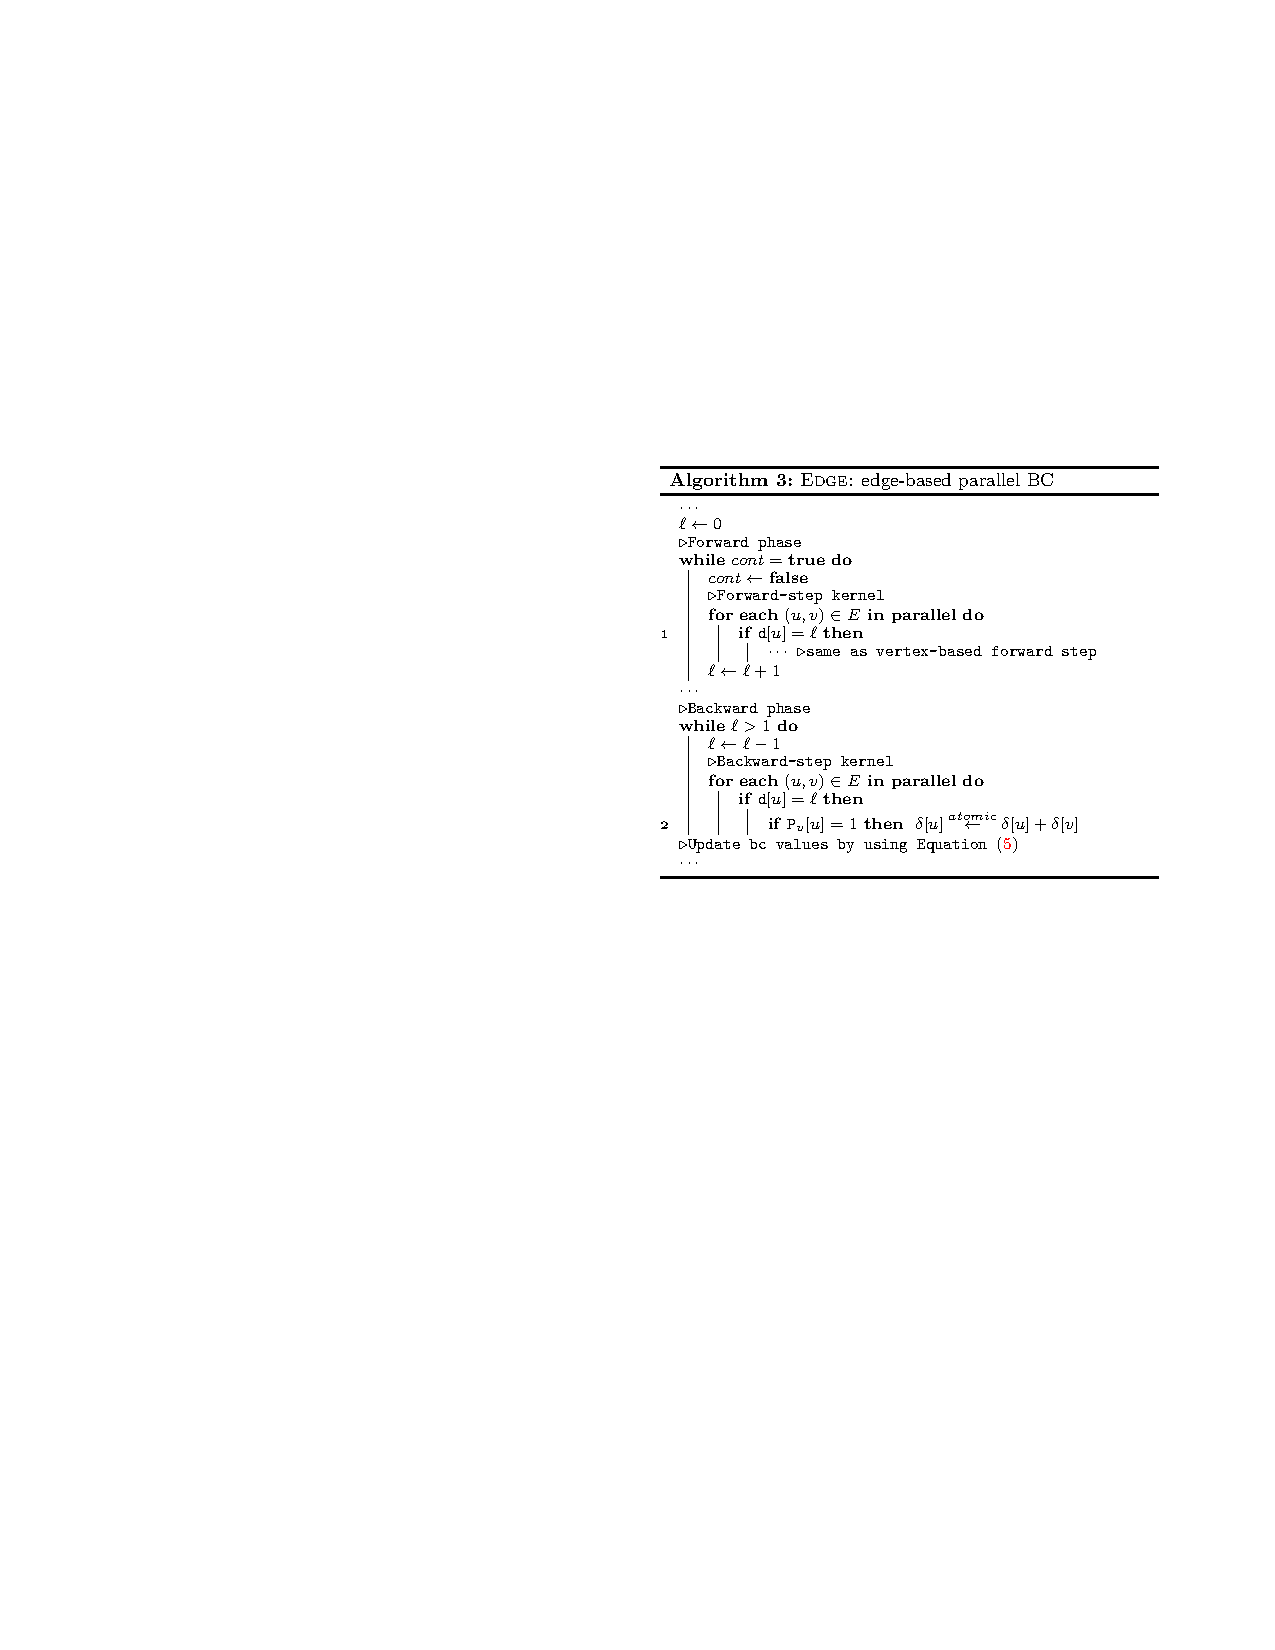
\includegraphics[width=\textwidth, height=0.8\textheight, keepaspectratio]{imgs/gpu-algo-edge}
      \end{figure}
    \end{column}
  \end{columns}
  
\end{frame}


\begin{frame}
  \frametitle{Vertex virtualization}

  \begin{columns}[onlytextwidth]
    \begin{column}{0.5\textwidth}
      \begin{itemize}
        \item AKA, edge packing/batching, \\ hybrid between vertex- and edge-based
        \item Split high degree vertices into virtual ones with maximum degree $mdeg$
        \item Equivalently, pack up to $mdeg$ edges belonging to the same vertex together
        \item Very small $mdeg = 4$
        \item Need additional auxiliary maps
      \end{itemize}
    \end{column}

    \begin{column}{0.5\textwidth}
      \begin{figure}[t]
        \centering
        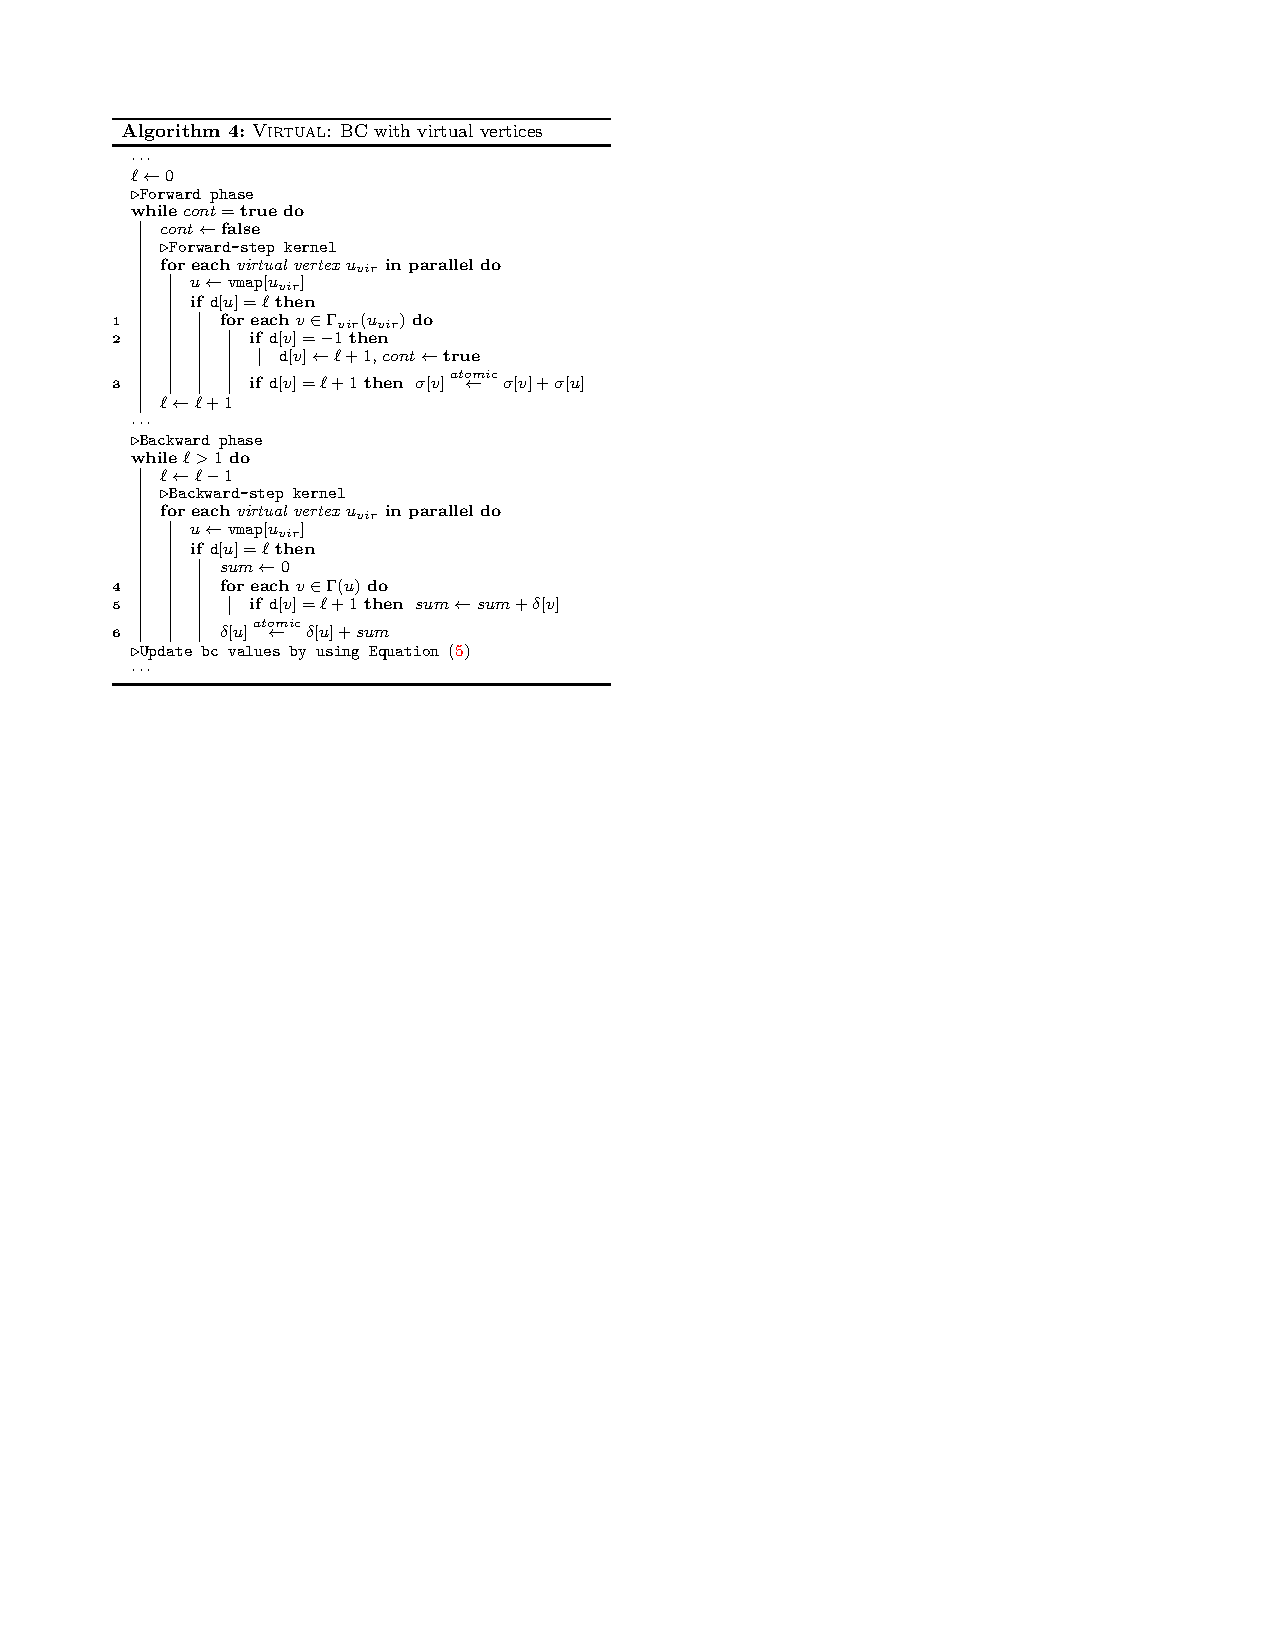
\includegraphics[width=\textwidth, height=0.8\textheight, keepaspectratio]{imgs/gpu-algo-hybrid}
      \end{figure}
    \end{column}
  \end{columns}
  
\end{frame}


\begin{frame}
  \frametitle{Benefits}
  
  \begin{itemize}
    \item Compared to vertex-based:
    \begin{itemize}
      \item Reduce load imbalance
    \end{itemize}
    \item Compared to edge-based:
    \begin{itemize}
    \item Reduce number of atomic operations
    \item Reduce memory footprint
    \end{itemize}
    \item Predecessors stored implicitly in the \spdag level (reduced memory usage)
    \item Memory layout can be further optimized to coalesce latency via \emph{striding}:
    \begin{itemize}
      \item Distribute edges to virtual vertices in round-robin
      \item When accessed in parallel, they create faster sequential memory access pattern
    \end{itemize}
  \end{itemize}
\end{frame}


\begin{frame}
  \frametitle{Results}

  \begin{figure}[t]
    \centering
    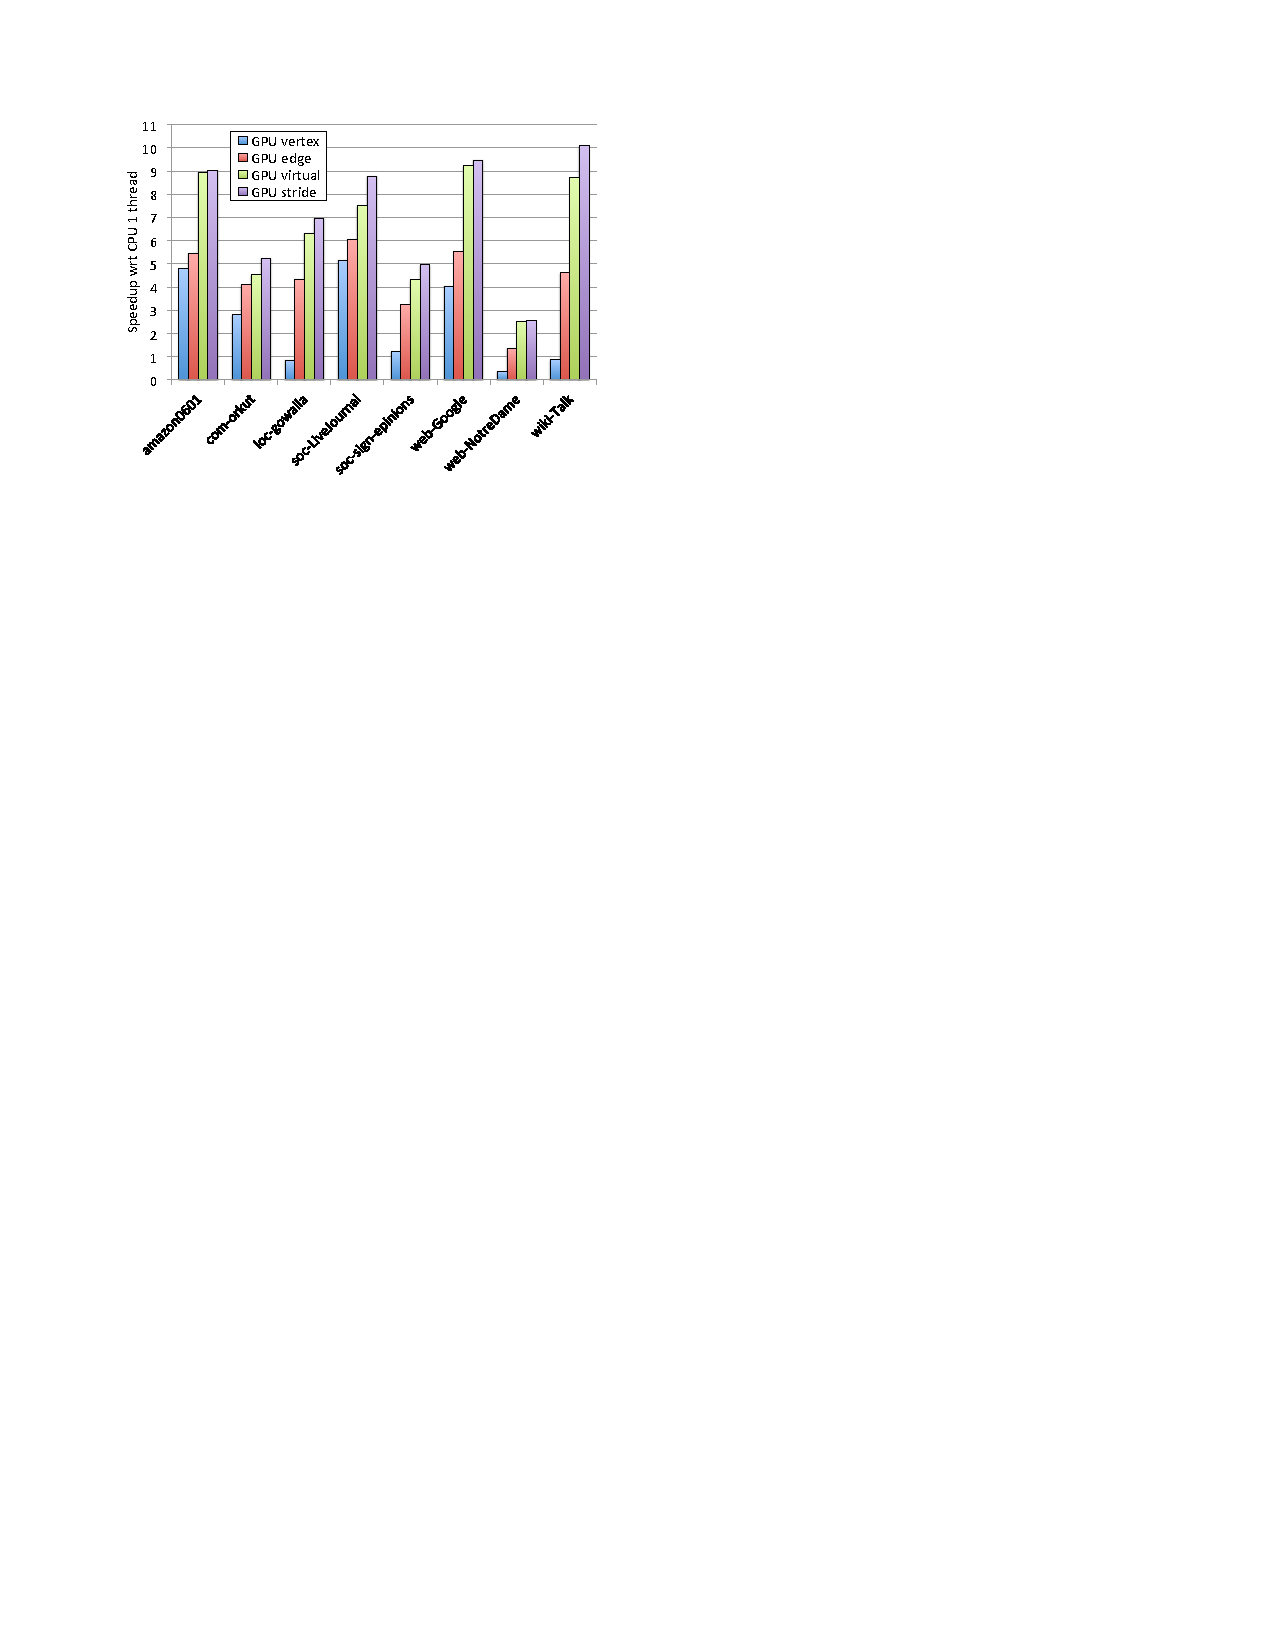
\includegraphics[width=\textwidth, height=0.6\textheight, keepaspectratio]{imgs/gpu-results1}
    \caption{Speedup over Brandes' on CPU on real graphs with 32-core GPU ($s= 1k, \ldots, 100k$)}
  \end{figure}
  
  \begin{itemize}
    \item Results computed only on a sample of sources and extrapolated linearly
  \end{itemize}
\end{frame}


%\begin{frame}
%  \frametitle{Results}
%
%  \begin{figure}[t]
%    \centering
%    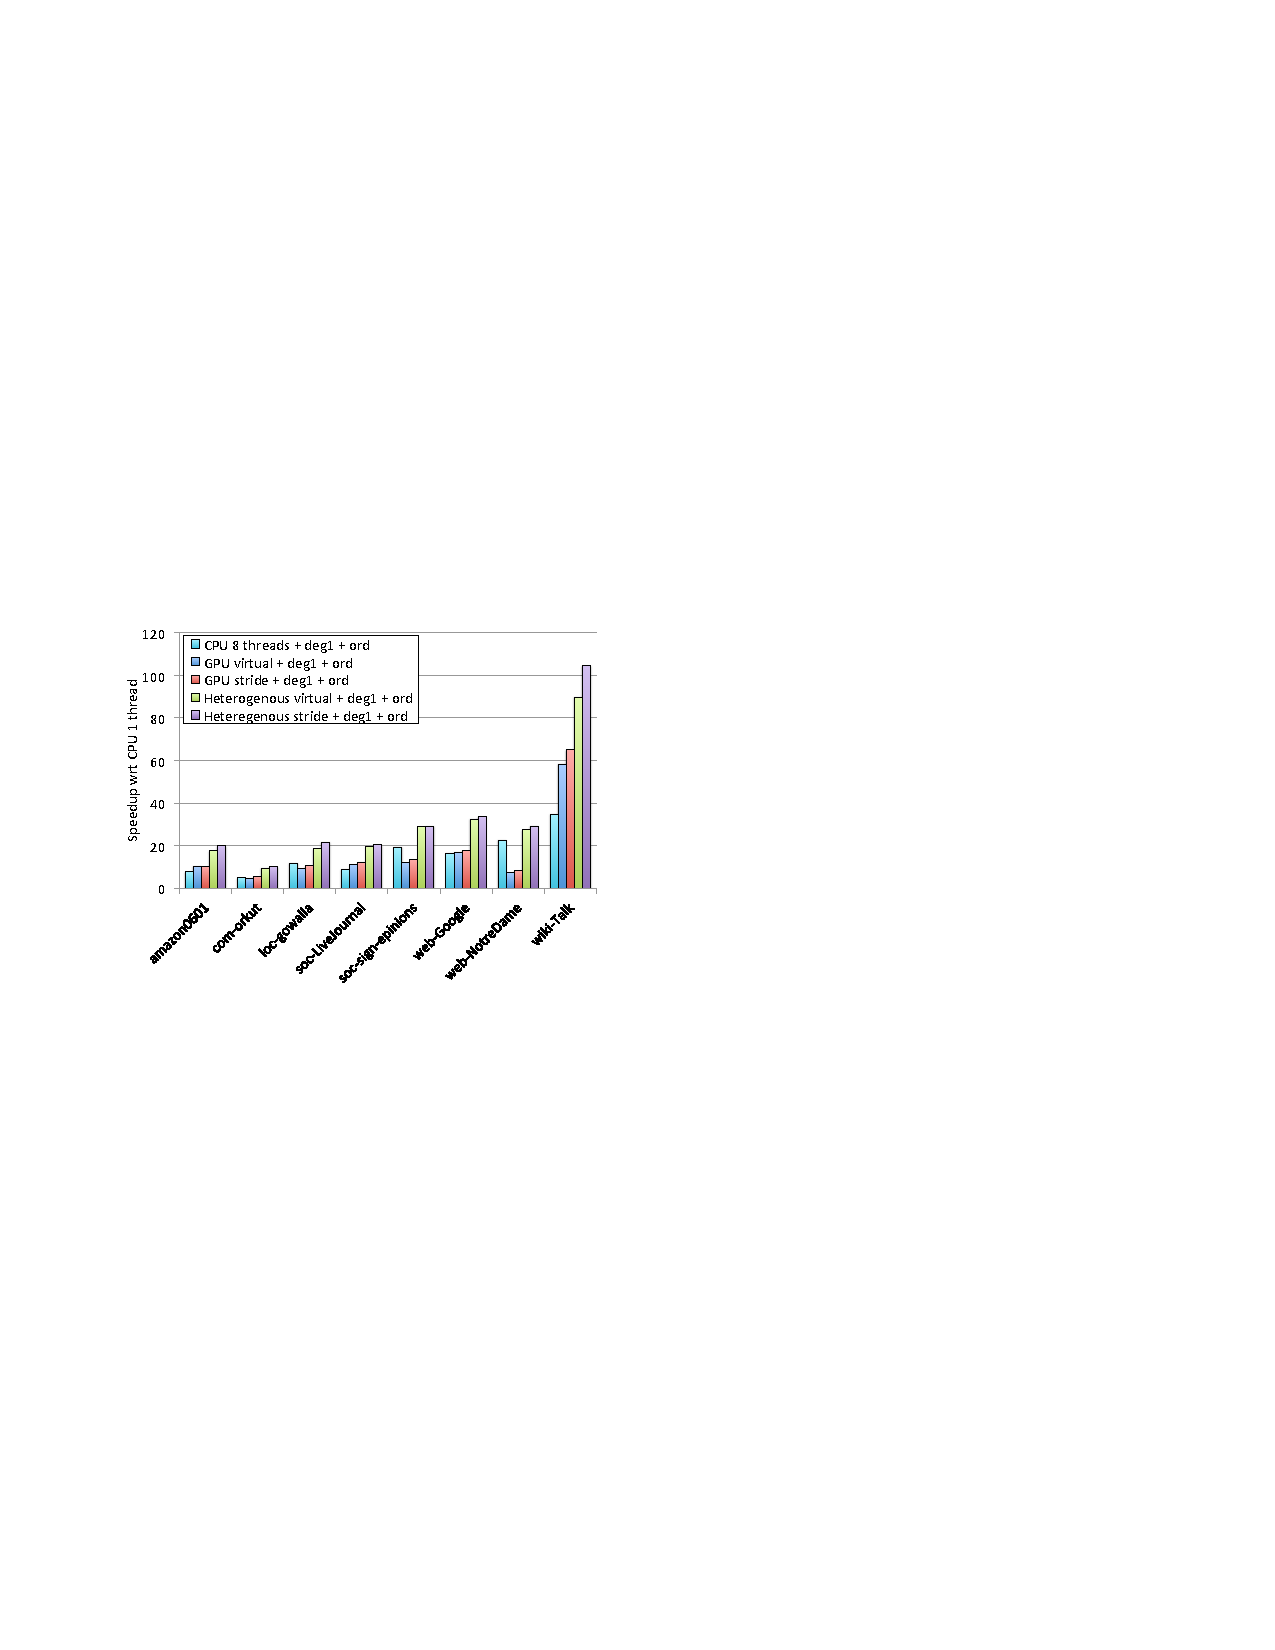
\includegraphics[width=\textwidth, height=0.6\textheight, keepaspectratio]{imgs/gpu-results2}
%    \caption{Speedup over Brandes' on CPU on real graphs with 32-core GPU}
%  \end{figure}
%    
%\end{frame}


%% Kourtellis et al.
\begin{frame}
  \frametitle{Scalable Online Betweenness Centrality in Evolving Graphs}
  \centering
  \vfill
  {\huge N. Kourtellis, G. De-Francisci-Morales, F. Bonchi}
  \vfill
  {\large TKDE: IEEE Transactions on Knowledge and Data Engineering (2015)}
\end{frame}


\begin{frame}
  \frametitle{Intuition}

  \begin{itemize}
    \item Incremental, exact, space-efficient, out-of-core, parallel version of Brandes'
    \item Handles edge addition and removal
    \item Vertex and edge betweenness
    \item Scalable to graphs with millions of nodes
  \end{itemize}

\end{frame}


\begin{frame}
  \frametitle{Algorithm}

  \begin{itemize}
    \item Run a modified Brandes' on the initial graph
    \item Keep track of \dist, \paths, \dep in a \spdag (no \pred)
    \item On edge update, adjust the \spdag and update \betw
  \end{itemize}
  
  \begin{figure}[t]
    \centering
    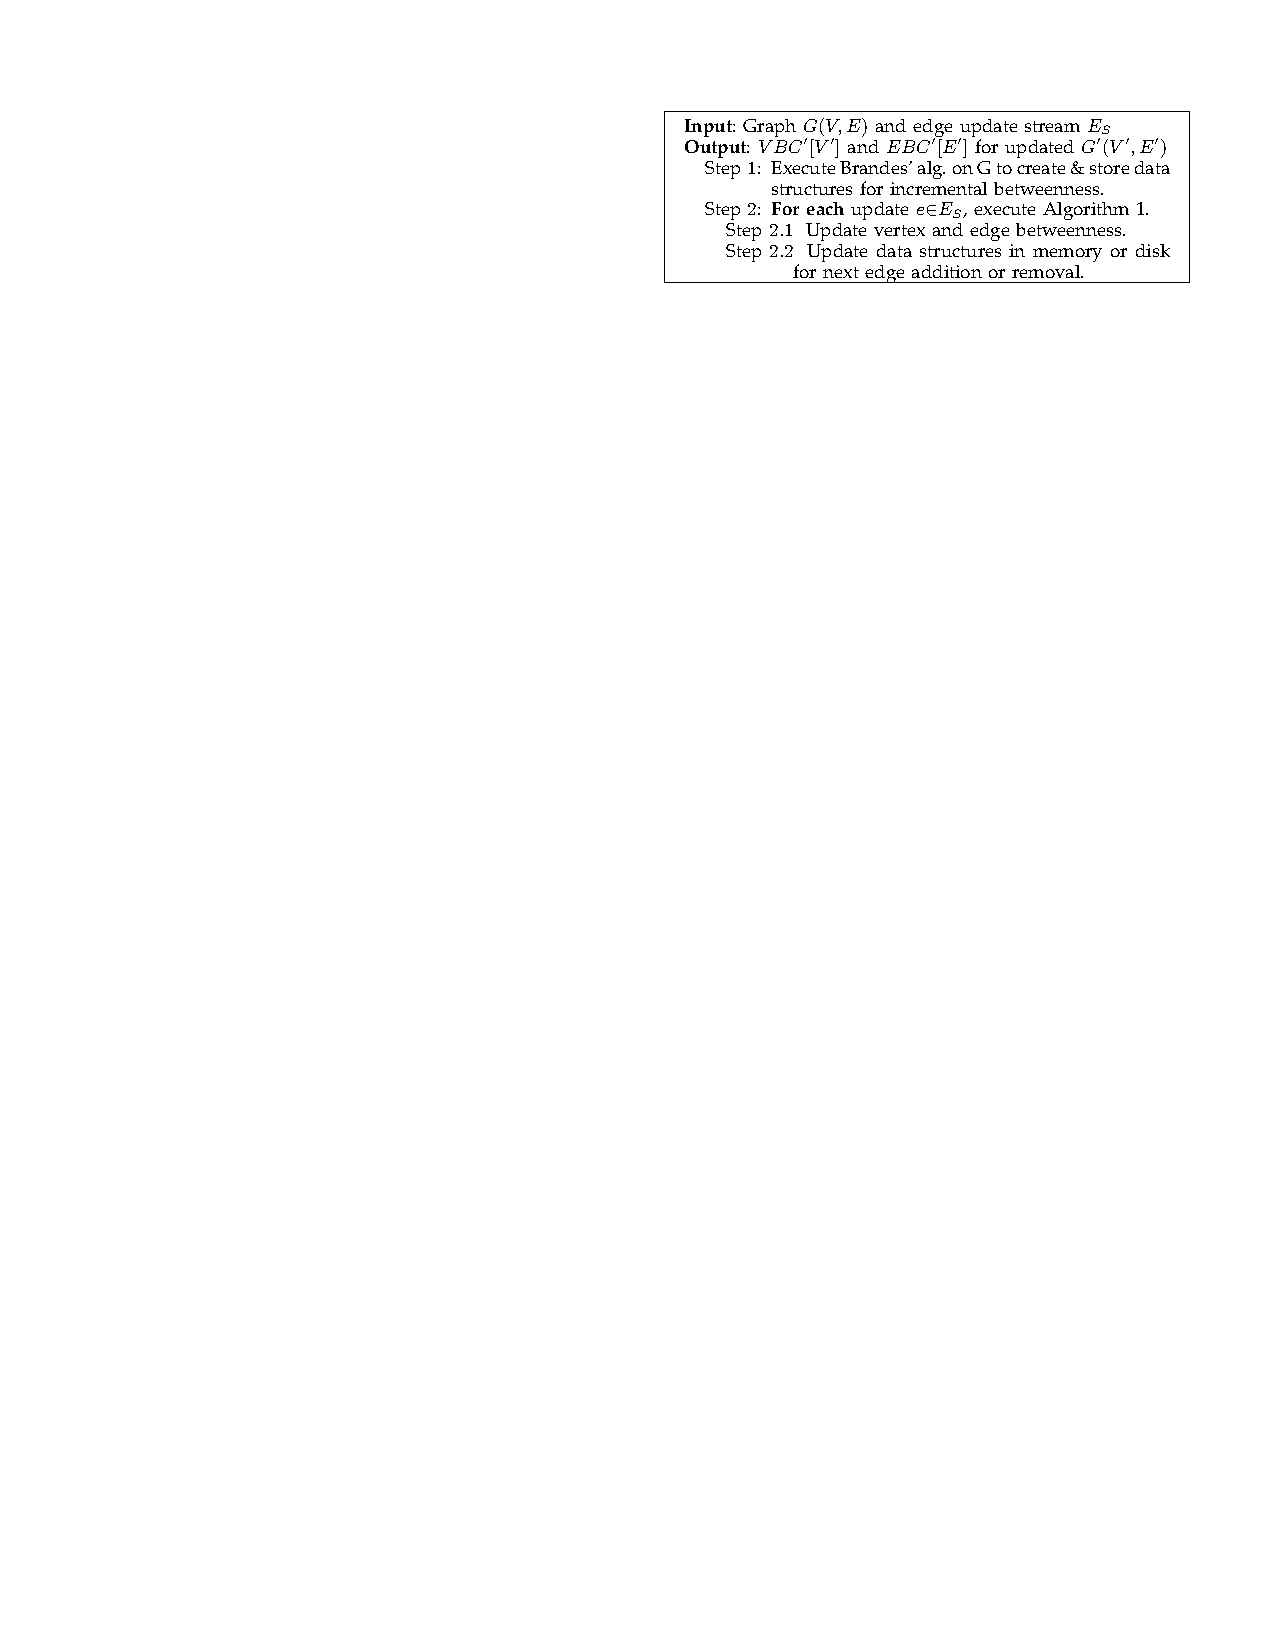
\includegraphics[width=\textwidth, height=0.6\textheight, keepaspectratio]{imgs/kdb-algo}
  \end{figure}

\end{frame}


\begin{frame}
  \frametitle{Data structure}

  \begin{itemize}
    \item $\spdag_s$ for each source $s \in V$
    \item \spdag contains \dist, \paths, \dep for each other vertex $t \in V$
    \item No predecessors \pred, re-scan neighbors and use \dist to find them
    \begin{itemize}
      \item Save memory - space complexity $O(n^2)$
      \item Fixed size data structure - efficient out-of-core management
      \item Same time complexity $O(nm)$ - in practice, makes the algorithm faster
    \end{itemize}
  \end{itemize}

\end{frame}


\begin{frame}
  \frametitle{Pivot}

  \begin{itemize}
    \item When adding or removing an edge, consider $dd = |d_{su} - d_{sv}|$
    \item Three cases: $dd=0$, $dd=1$, $dd>1$ (analogous to Green et al.)
    \item Last case $dd>1$ hardest - structural changes in \spdag
    \item Find \emph{pivots} to discover structural changes
  \end{itemize}
  
  \begin{definition}[Pivot]
Let $s$ be the current source, let $\dist$ and $\dist'$ be the distance before and after an update, respectively, we define \emph{pivot} a vertex $p \mid \dist(s,p) = \dist'(s,p) \wedge \exists \, w \in \neighbors(p)$$: \dist(s,w)$$\neq$$\dist'(s,w)$.
  \end{definition}
  
  \begin{itemize}
    \item Pivots' distance unchanged $\rightarrow$ use as starting points to correct distances
  \end{itemize}

\end{frame}


\begin{frame}
  \frametitle{Finding pivots}

  \begin{itemize}
    \item Addition - pivots in sub-dag rooted in $u_L = v$ 
    \item Nodes moved closer must be reachable from $u_L$
    \item Can be found during exploration while fixing \paths
  \end{itemize}
  \begin{itemize}
    \item Removal - pivots may be anywhere
    \item Need one exploration to find them
    \item Need separate exploration from found pivots to correct distances
  \end{itemize}

  \begin{figure}[t]
    \centering
    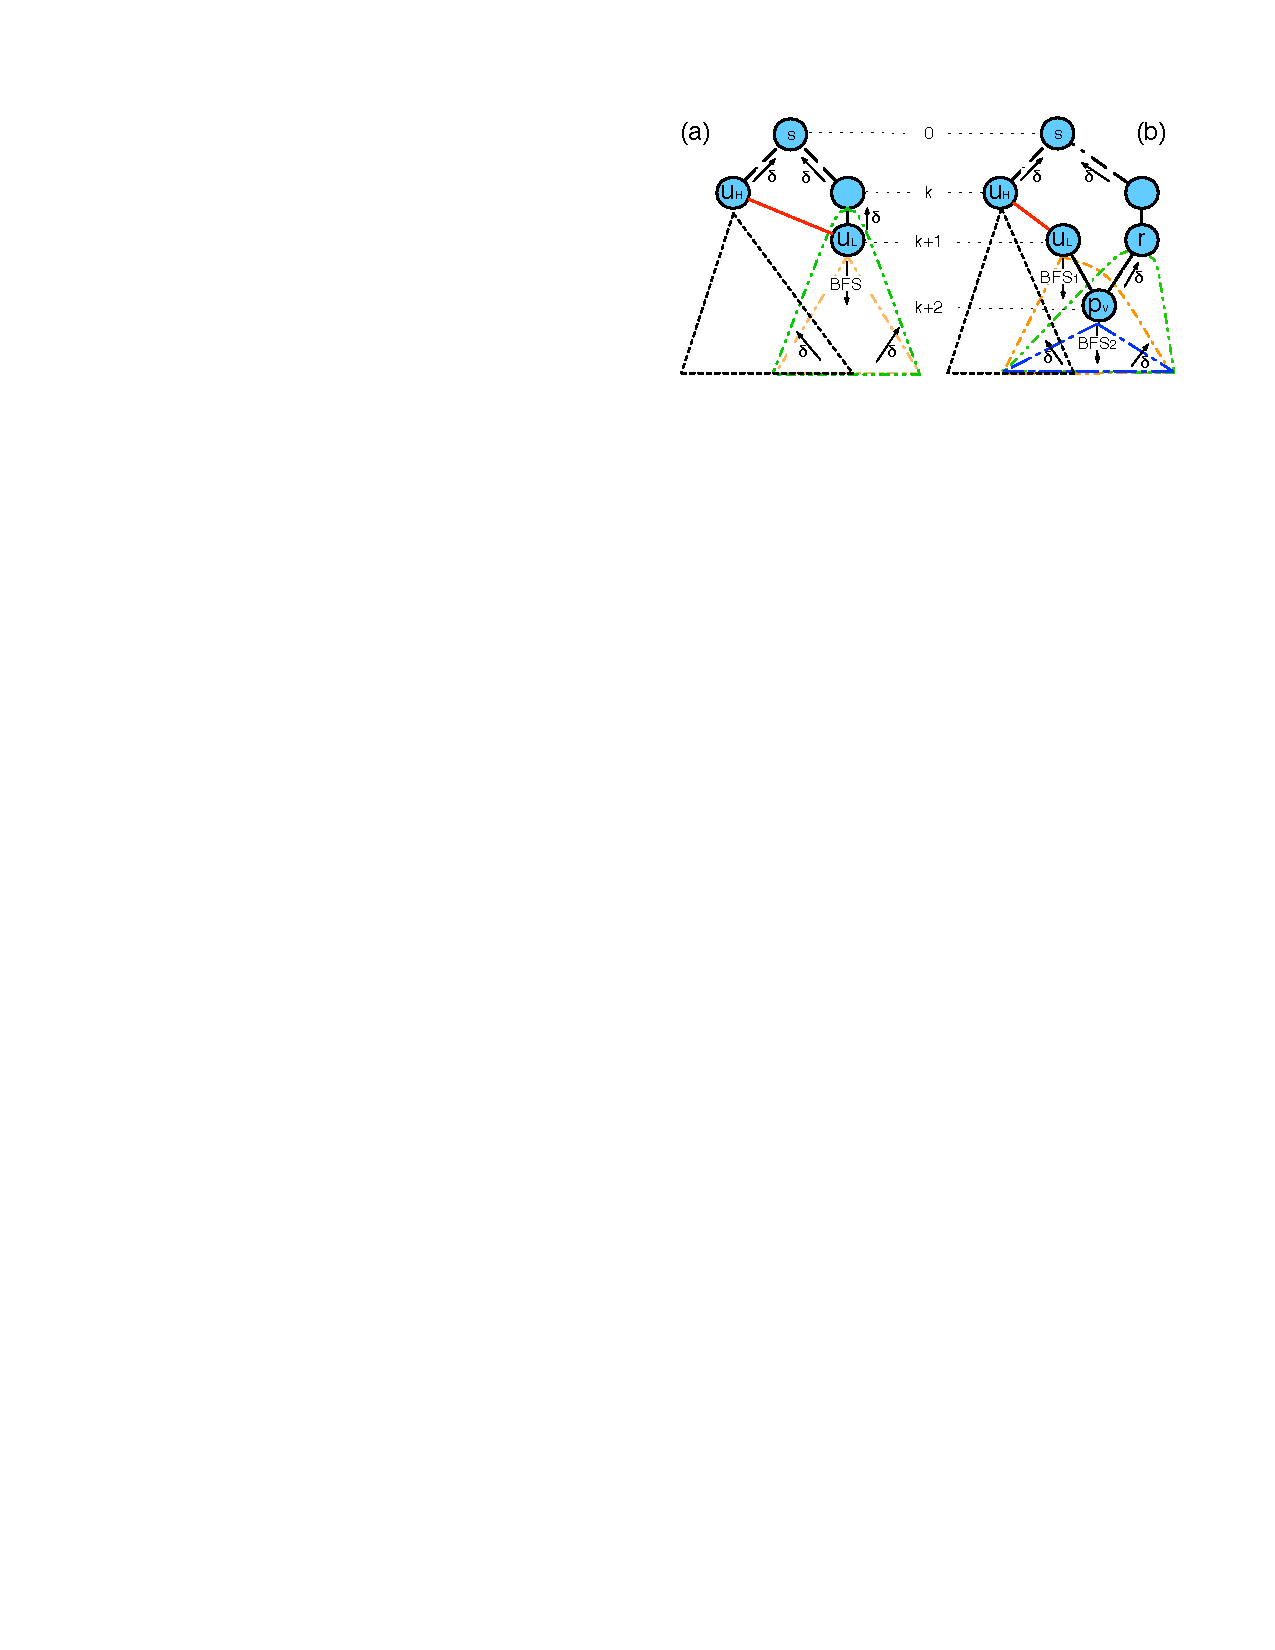
\includegraphics[width=\textwidth, height=0.5\textheight, keepaspectratio]{imgs/kdb-bfs}
  \end{figure}

\end{frame}


\begin{frame}
  \frametitle{Structural changes}

  \begin{figure}[t]
    \centering
    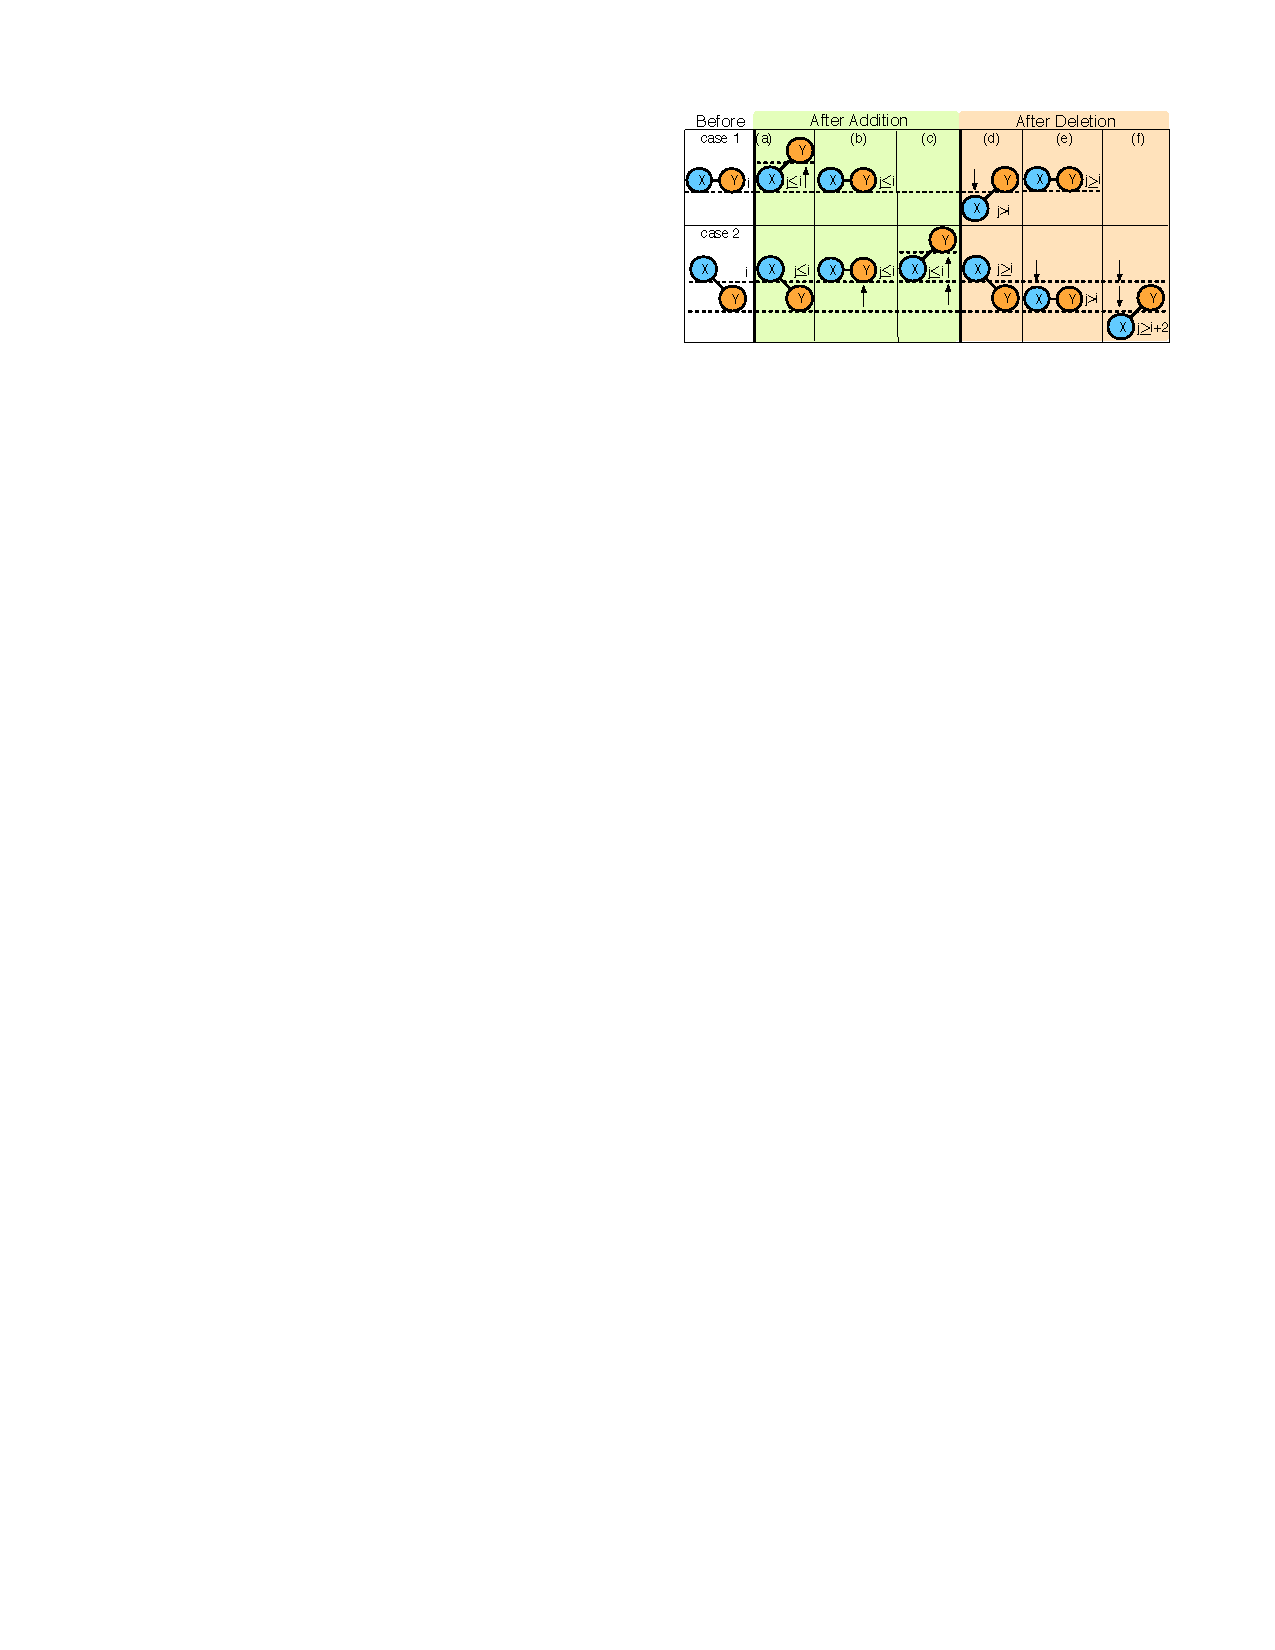
\includegraphics[width=\textwidth, height=0.5\textheight, keepaspectratio]{imgs/kdb-cases}
  \end{figure}

  \begin{itemize}
    \item Consider $x \in \neighbors(y)$, $x$ can either be a sibling or a predecessor of $y$
    \item Each case requires slightly different combination of corrections for \dist, \paths, \dep
    \item $y$ is pivot in 1d, 2e, 2f
    \item Removal for case 1d can be optimized (pivot $y$ is sibling of $x$)
  \end{itemize}
  
\end{frame}


\begin{frame}
  \frametitle{Scalability}

  \begin{itemize}
    \item Out-of-core
    \item In-place update - minimize writes
    \item Columnar storage - skip if $dd=0$
    \item Parallelization
  \end{itemize}
  
\end{frame}


\begin{frame}
  \frametitle{Results}

  \begin{itemize}
    \item 
  \end{itemize}
\end{frame}


\begin{frame}
  \frametitle{Results}

  \begin{itemize}
    \item 
  \end{itemize}
\end{frame}


\begin{frame}
  \frametitle{Conclusions}

  \begin{itemize}
    \item 
  \end{itemize}
\end{frame}

